\documentclass[defaultstyle,11pt]{thesis}

\usepackage{amssymb}		% to get all AMS symbols
\usepackage{amsmath}		% to get equations to work right
\usepackage{graphicx}		% to insert figures
\graphicspath{{../}{Trap/}}
\usepackage[pagebackref = true]{hyperref}		% PDF hyperreferences?? [backref=none]
\usepackage{natbib}
\usepackage{array}
\newcolumntype{L}[1]{>{\raggedright\let\newline\\\arraybackslash\hspace{0pt}}m{#1}}
\newcolumntype{C}[1]{>{\centering\let\newline\\\arraybackslash\hspace{0pt}}m{#1}}
\newcolumntype{R}[1]{>{\raggedleft\let\newline\\\arraybackslash\hspace{0pt}}m{#1}}
\usepackage{caption}
\setcitestyle{numbers,square,comma}
\usepackage[usenames,dvipsnames]{color}
%% To make \href colors more decent:
\definecolor{MyDarkBlue}{rgb}{0,0.1,0.7}
\hypersetup{pdfborder={0 0 0},colorlinks,breaklinks=true,
  urlcolor={MyDarkBlue},citecolor={MyDarkBlue},linkcolor={MyDarkBlue}
}
\renewcommand{\thefootnote}{\alph{footnote}}	
\title{a}
\abstract{a}
\author{a}{a}
\otherdegrees{a}
\degree{a}{a}
\dept{a}{a}
\advisor{a}{a}
\reader{a}
\readerThree{a}
\SuspendPrologue
\begin{document}
\input macros.tex

\chapter{Molecular Trapping}

Some of the earliest successful trapping of neutral molecules began with CaH in John Doyle's group in a dilution fridge with $^3$He buffer~\cite{Weinstein1998}.
Stark decelerated and electrostatic trapped ammonia followed soon later~\cite{Bethlem2000trap}.
Since then extensions to many species have occurred. 
In this chapter we focus on OH molecules, whose strong Stark shift to mass ratios make them favorable for attempts to attain high enough densities to observe collisions between members of the ensemble.

%% SECTION HISTORY OF OH TRAPS
%% SECTION HISTORY OF OH TRAPS
\section{History of OH traps}

%Trap History Table
\renewcommand{\arraystretch}{1.5}
\begin{table}[t!]
\centering
\caption{
The Ye Group Molecule trapping endeavor.\label{trappingtable}
}
\label{tab:rates}
\begin{tabular}{ L{2.5cm} | C{4.5cm} C{2.5cm} C{4.5cm} }
Name & Type & Depth (mK) & Uses \\
\hline\hline
MET 	& Magnetic Quadrupole, Electric Hexapole & 250 	& First Demonstration~\cite{Sawyer2007} 	 \\
\hline
Ring 		& Magnetic Quadrupole				& 100 	& He, D$_2$, ND$_3$ Collisions~\cite{Sawyer2008,Sawyer2011} \\
\hline
Ring 		& Above, but new mounts				& 100 	& E-field Induced Collisions,  Evaporation~\cite{Stuhl2012uwave,Stuhl2012evap,Stuhl2013} \\
\hline
Tricycle 	& Magnetic Quadrupole 				& 300 	& 10x density, spin-flip loss \\
\hline
Pin  		& 2D Magnetic and Electric Quadrupoles 	& 500 	& Solved spin-flip loss~\cite{Reens2017}\\
\hline
Cryocycle 	& Magnetic Quadupole 				& 200 	& Lifetime, Fluorescence Enhancements\\
\end{tabular}
\end{table}

The history of OH trapping in the Ye group has grown substantial enough to warrant a tabular environment~\ref{trappingtable}. 
Each attempt has brought new challenges and experiences, and steady progress has been made in a number of key areas.
The Magnetoelectrostatic Trap (MET) installed during Brian Sawyer's time~\cite{Sawyer2007} was a heroic first attempt that included a few-turn magnetic coil run at a startling $1400$~A, and $2000$~A briefly during loading.
Later it was decided to trade the role of the fields used for loading, and great gains in magnetic field strength and simplicity were attained by switching to permanent magnets with the ``Ring'' trap~\cite{Sawyer2011}.
A key improvement occurred when it was discovered that patch charges on the Ultem mounts originally used for affixing the magnetic trap to the Stark decelerator could have a significant impact on spectroscopic efforts~\citep[Fig.~6]{Stuhl2012uwave}.
This was addressed by designing primarily stainless steel mounts, so that molecules only had line of sight to grounded conductors, although still with insulators installed between the decelerator and trap but relocated elsewhere.

% SECTION TRICYCLE OVER RING TRAP
% SECTION TRICYCLE OVER RING TRAP
\section{Tricycle over Ring Trap}

In pursuit of increases in density and molecule number, an iteration on the Ring trap was performed, dubbed the ``Tricycle'' trap due to the three rectangles formed when examining planar cuts through the ring and rear magnets used to generate the trap, see Fig.~\ref{ringtricyclefigure}.
This was first installed in 2014, and improved on the Ring trap in several key ways:
\begin{enumerate}
\item Replaced rear ring with its core, removing an outer toroidal trap and tripling depth.
\item Significantly improved loading dynamics.
\item Increased trap gradient, thanks to a $\sim 40\%$ reduction in size.
\end{enumerate}

\begin{figure}[t!]
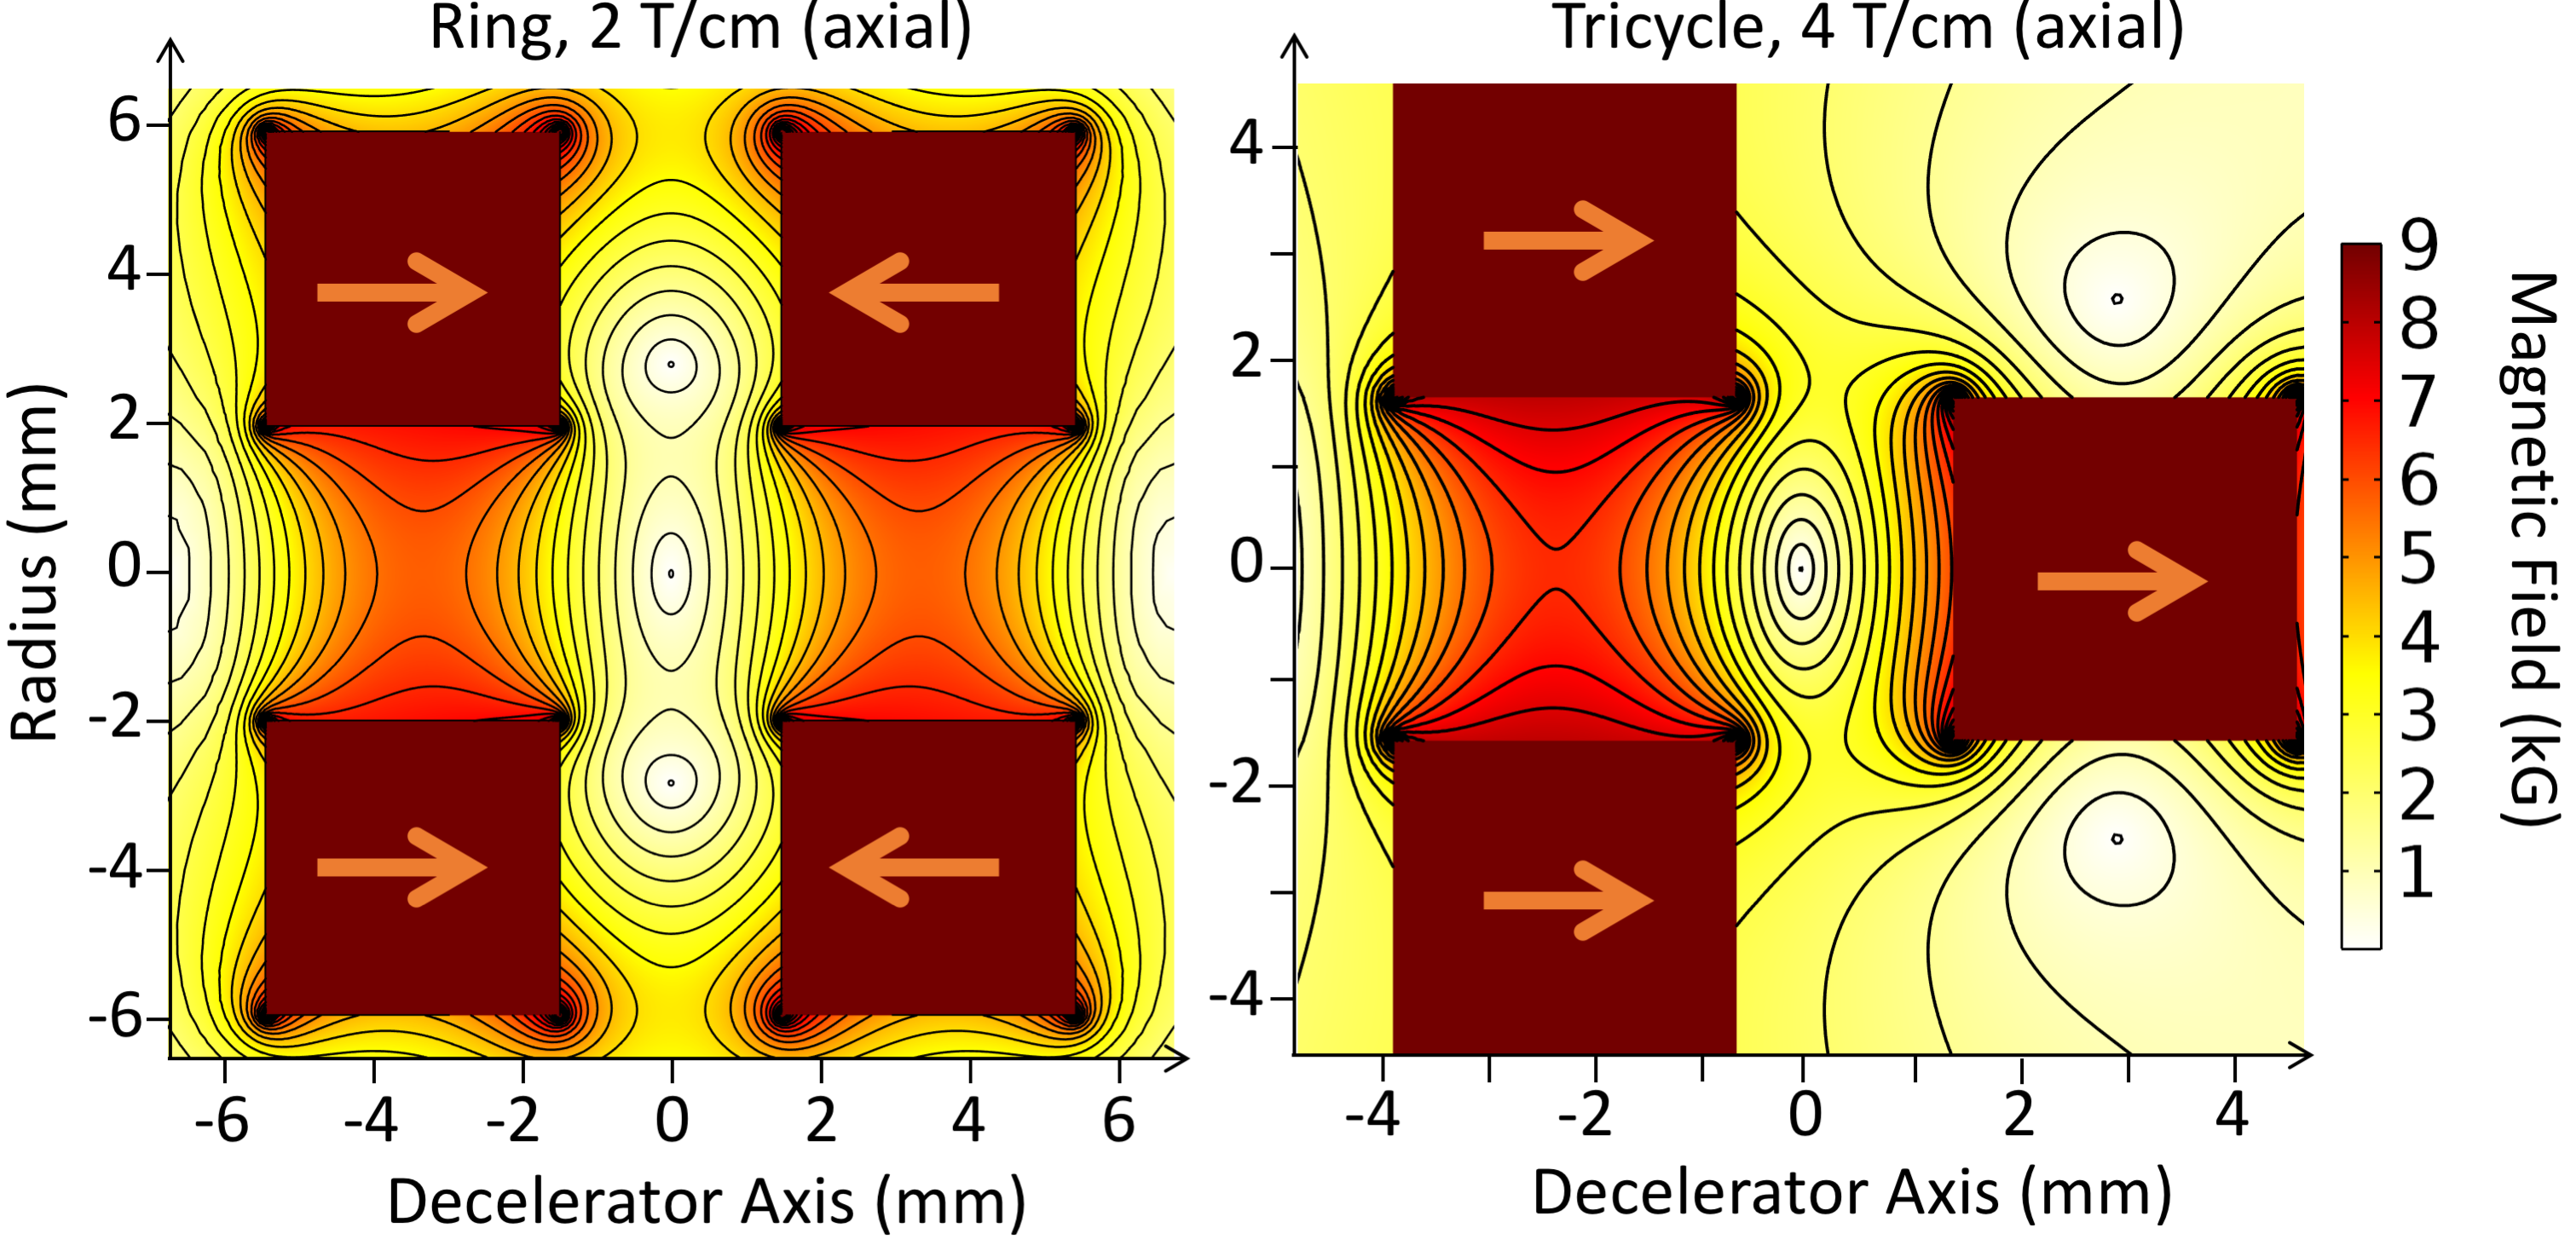
\includegraphics[width=\linewidth]{RingTricycle.png}
\caption[Ring and Tricycle Trap Comparison]{\label{ringtricyclefigure}
Cross Sections including the cylindrically symmetric axis for both the Ring and Tricycle traps. Arrows indicate magnetization directions up to an overall sign. Magnetic trapping fields are shown, demonstrating the destabilization of the toroidal minimum of the Ring trap. Contours every $500$~G. Steel mounting electrodes are not shown in either case, but are installed on the outer diameter of the magnets and affixed to them with setscrews.
}
\end{figure}

%SUBSECTION TOROIDAL DESTABILIZATION
\subsection{Toroidal Destabilization}

This first achievement was one of the primary goals of the iteration, since the influence of the toroidal minimum present in the Ring trap was difficult to ascertain. 
Molecules ought to have been able to explore the toroidal region, but based on the observed distribution of molecules as a function of magnetic field, they did not appear to be doing so for unknown reasons.
At the time it was highly desirable to be able to perform the same evaporation type experiments, but in a geometry without a toroidal minimum.
The removal of the toroidal minimum can be best understood by thinking about the traps using the principle of superposition.
The Ring trap may be thought of as the result of superposing two different quadrupole traps, one formed by cylinders of diameter given by the ID of the rings, and the other formed by cylindrical magnets of diameter given by the OD of the rings.
The smaller quadrupole trap is nice and tight, but the magnets block the beam path.
The larger trap is larger and weaker, and its field lines move in the opposite direction, since its magnets are oppositely magnetized relative to the smaller quadrupole trap (so that they cancel each other out in the centers of the rings, allowing molecules to pass through).
The larger trap works against the smaller, but is much weaker than it at least near the center of the geometry, so that the smaller remains somewhat tight near the trap center.
Further outside, where the fields generated by the smaller quadrupole trap are less significant, the outer quadrupole dominates, creating the outer toroidal minimum.
If instead of overlapping a larger quadrupole trap with the smaller, we just overlap a single disk magnet, then no significant outer trap is created, just as in the Tricycle trap.

In fact, in the limit of large OD of the single ring magnet of the Tricycle trap, the geometry exactly approaches that of a pair of small disk magnets, but with the crucial modification of an entry hole for the molecules to be delivered.
This is because for a disk magnet, the on-axis magnetic field is given by:
\begin{equation}
B(z) = \frac{1}{2}B_r\left(\frac{z+t}{\sqrt{R^2+(z+t)^2}} - \frac{z-t}{\sqrt{R^2+(z-t)^2}}    \right),
\end{equation}
where $B_r$ is the remanent flux density of the permanent magnet, $t$ is its half thickness, and $z$ the distance from the magnet center, and $R$ gives the cylinder radius. In the limit of large $R$ we obtain:
\begin{equation}
B(z) = \frac{1}{2}B_r\left( \frac{z+t}{R+(z+t)^2/2R)}  - \frac{z-t}{R+(z-t)^2/2R)}   \right),
\end{equation}
and taking it to cubic order:
\begin{eqnarray}
B(z) &=& \frac{1}{2}B_r\left( \frac{z+t}{R} - \frac{(z+t)^3}{2R^3}  - \frac{z-t}{R} + \frac{(z-t)^3}{2R^3}   \right)\\
&=& \frac{1}{2}B_r\left(\frac{2t}{R} - \frac{3z^2t}{R^3} + \frac{t^3}{R^3} \right).
\end{eqnarray} 
So we see that as $R$ grows, $B(z)$ shrinks close to the magnet with $1/R$, but the flatness of the field increases, so that the term proportional to $z^2t/R^3$ which describes the second order fall off of the field away from the magnet reduces as $1/R^3$.

%SUBSECTION LOADING IMPROVEMENTS
\subsection{Loading Improvements}

The Tricycle trap features very significant loading improvements over the Ring trap, although the precise extent is difficult to pin down. 
The main reason for an expectation of improvement lies in the phase space dynamical behavior of the two geometries.
In analyzing any trap loading scenario, it is important to pursue the analysis with both intuition and simulation.
The latter on its own will lack the guidance necessary for truly identifying an optimal scenario, while the former is unlikely to be able to fully disentangle interdependent factors influencing performance.

On the intuitive side, it is useful to use the same reasoning as in the decelerator by focusing on phase stability.
The loading fields generated by charging up the surfaces of the ring magnets in the Ring trap are mirror symmetric about the center of the Ring trap.
This means that if a loading sequence is designed so that the synchronous molecule ends up exactly in the trap center, the synchronous molecule will be required to roll up to the top of a hill and then stop there. 
Molecules with slightly more forwards velocity than the synchronous molecules will end up quite a ways down the other side of the hill by the time the loading fields are switched off, and vice versa.
In layman's terms, longitudinal phase stability during loading requires that the loading be performed on a slope, not a peak.

It is possible to generalize these ideas further, while still remaining in the intuitive domain.
If it is true that the loading fields ought to feature a slope at the location of the trap center where the synchronous molecule comes to rest, what is the ideal value for that slope?
Also, is there a similar ideal value for the slope of the loading fields in the region in front of and beyond the trap center?
We can answer these questions with a simplified thought experiment, refer to Fig.~\ref{LoadingRotation}.
Suppose we have a population experiencing a harmonic trapping potential with a characteristic width $\delta z$ in real space and $\delta v$ in velocity space, and centered at $z_0=0$ and $v_0 > 0$.
One way to controllably transfer this population to $v_0=0$ without unwanted stretching of the population would be to load it into a much larger harmonic potential with oscillation frequency $\omega$ centered at $z=0$ and $v=0$.
Because harmonic potentials always execute rotations in phase space with ellipticity controlled by their oscillation frequency, the population would then be smoothly transferred over the course of a quarter oscillation to be centered at $z = v_0/\omega$ and $v=0$, with widths $\omega\delta z$ and $\delta v/\omega$.
If $\omega$ is chosen equal to $\delta v/\delta z$, i.e. to have the same strength as the trapping potential prior the initiation of the loading sequence, then the original widths in position and velocity are precisely maintained.
On the other hand, $\omega$ could be tuned so as to optimize coupling between the initial traveling trapping potential and the trapping potential to be used after loading.

\begin{figure}[t!]
\centering
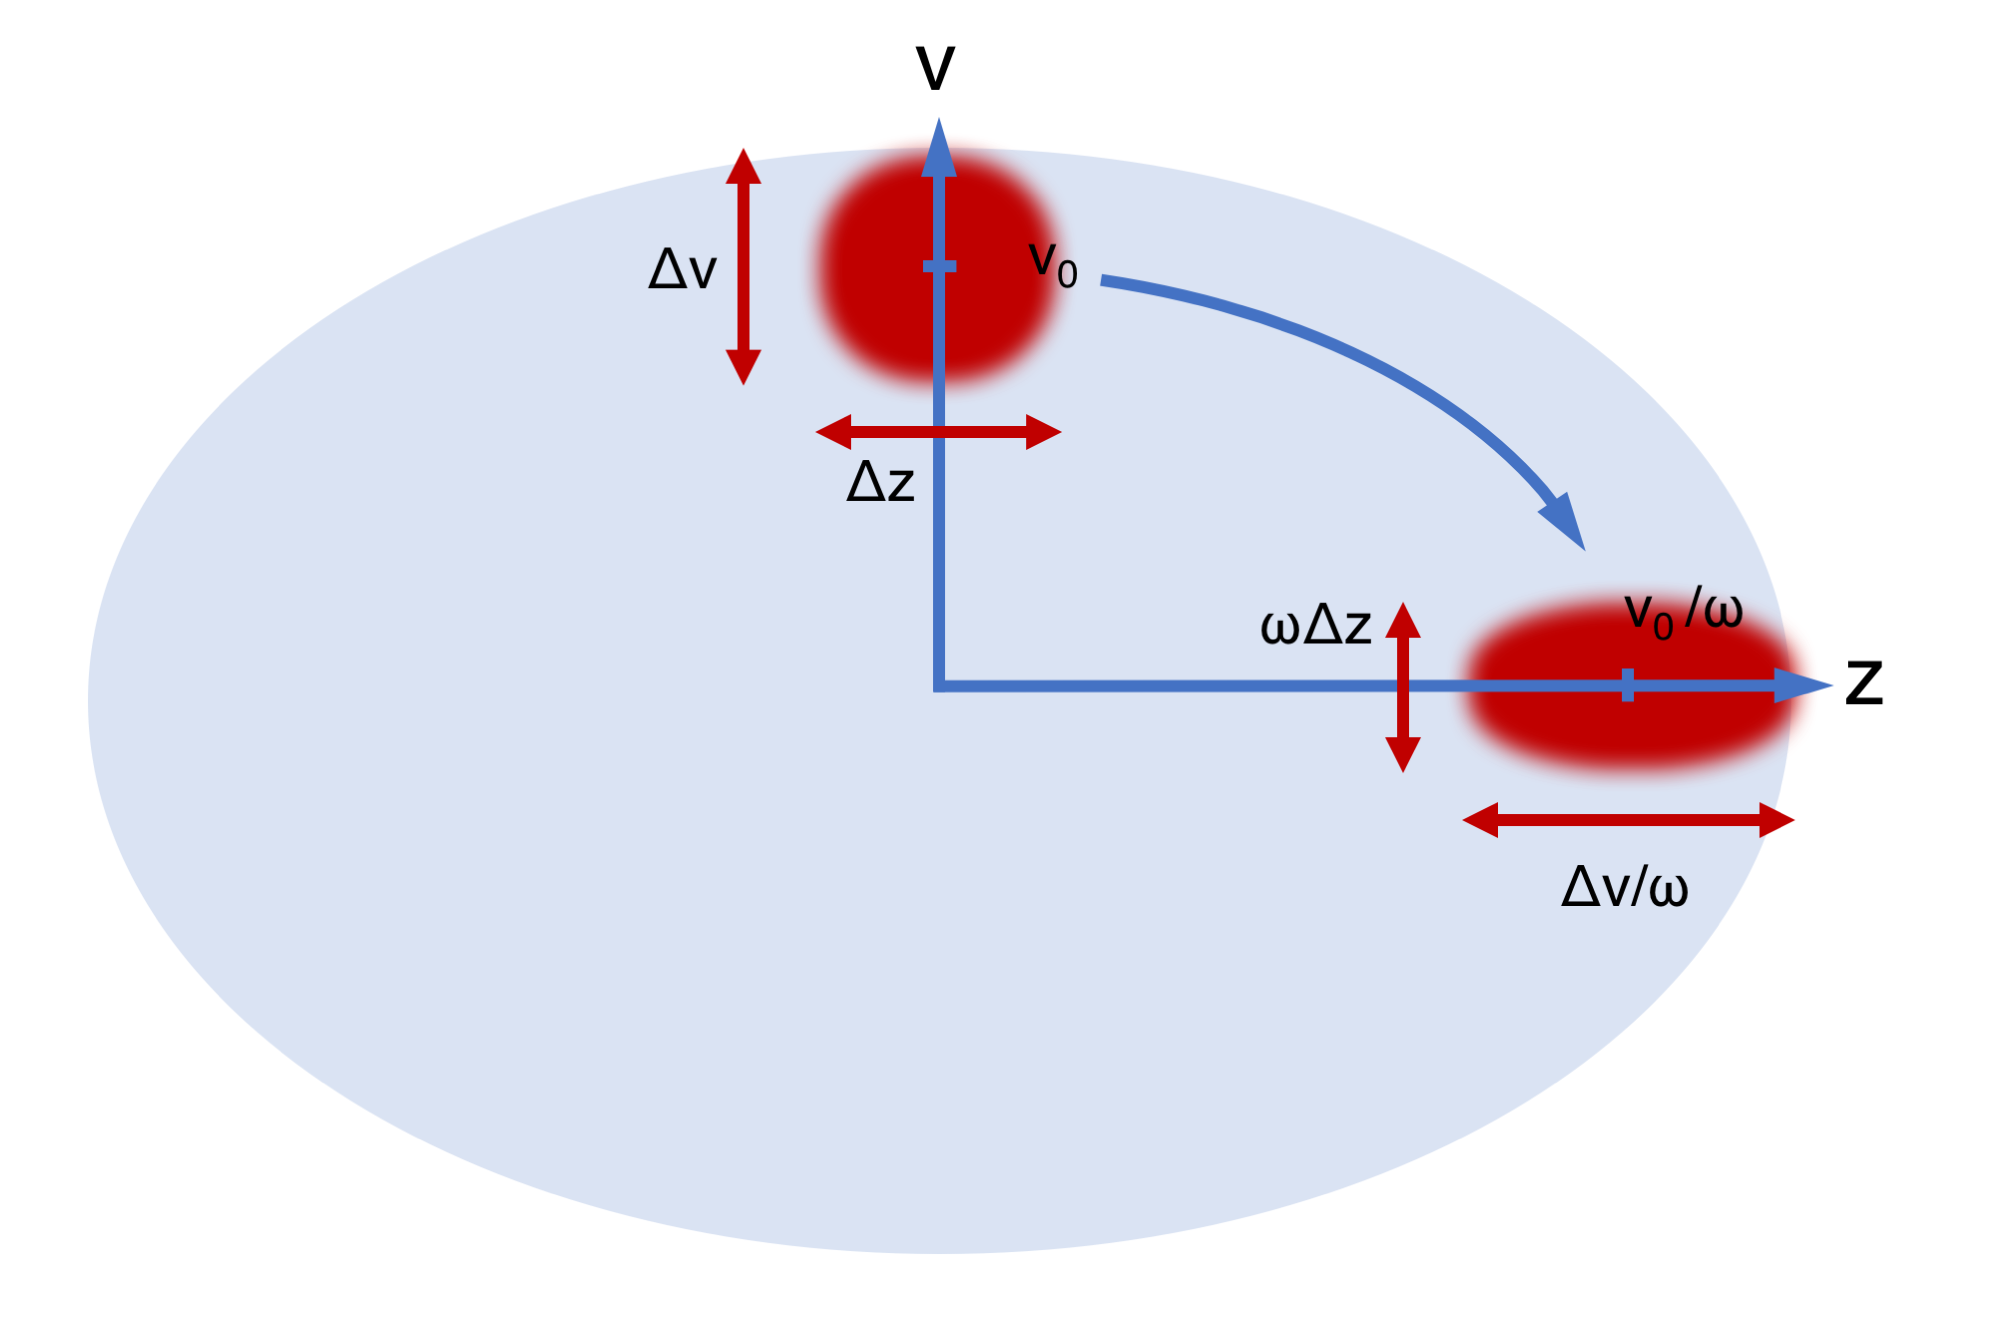
\includegraphics[width=10cm]{LoadingRotation.png}
\caption[Ideal Trap Loading as a Quarter Rotation]{\label{LoadingRotation}
Phase space diagram depicting the action of the ideal phase space conservative loading fields derived from a large external harmonic potential. The region of phase space acted on by the external potential is indicated as a light blue ellipse. The region of phase space populated initially is shown in red along the $v$ axis. The region populated after rotation is shown along the $z$ axis also in red. Widths and origins are as indicated.
}
\end{figure}

In addition to this harmonic loading potential, it would be ideal to also maintain a transverse trap simultaneously. 
The ideal fields would have a magnitude with the following spatial dependence:
\begin{equation}
|E(x,y,z)| = \frac{1}{2}m_{OH}\left(\omega_z^2z^2 + \omega_r^2r^2\right)
\end{equation}
where $\omega_z$ and $\omega_r$ are the longitudinal and transverse trap frequencies.
Neglecting the nonlinearity of the Stark shift for OH molecules close to zero field, such a harmonic potential could be generated transversely with a hexapole, but to do it simultaneously in the transverse and longitudinal directions would require an octupole moment, such as could be generated with three rings and two endcaps with the endcaps at $+V$, the outer rings grounded, and the inner one at $-V/2$ so as to approximate spherical boundary conditions following the second Legendre polynomial~\cite{jackson1999classical}.
This would of course be very unlikely to be able to be crammed into the small space between the end of a decelerator and a trap, and unlikely to be able to be charged up to a high enough potential energy for stopping an appreciable speed $v$.
It is much more likely that an efficient solution would be obtained by abandoning the harmonicity and instead focusing on the reduced criterion of loading fields that respect phase stability by having a slope at the location of what will be come the trap center and which also provide some transverse confinement.
The slope of the loading field at the location of the trap center would ideally match the slope that the ideal harmonic trap with frequency $\omega$ would have at that point, $m_\text{OH}\omega v_0$.

\begin{figure}[t!]
\centering
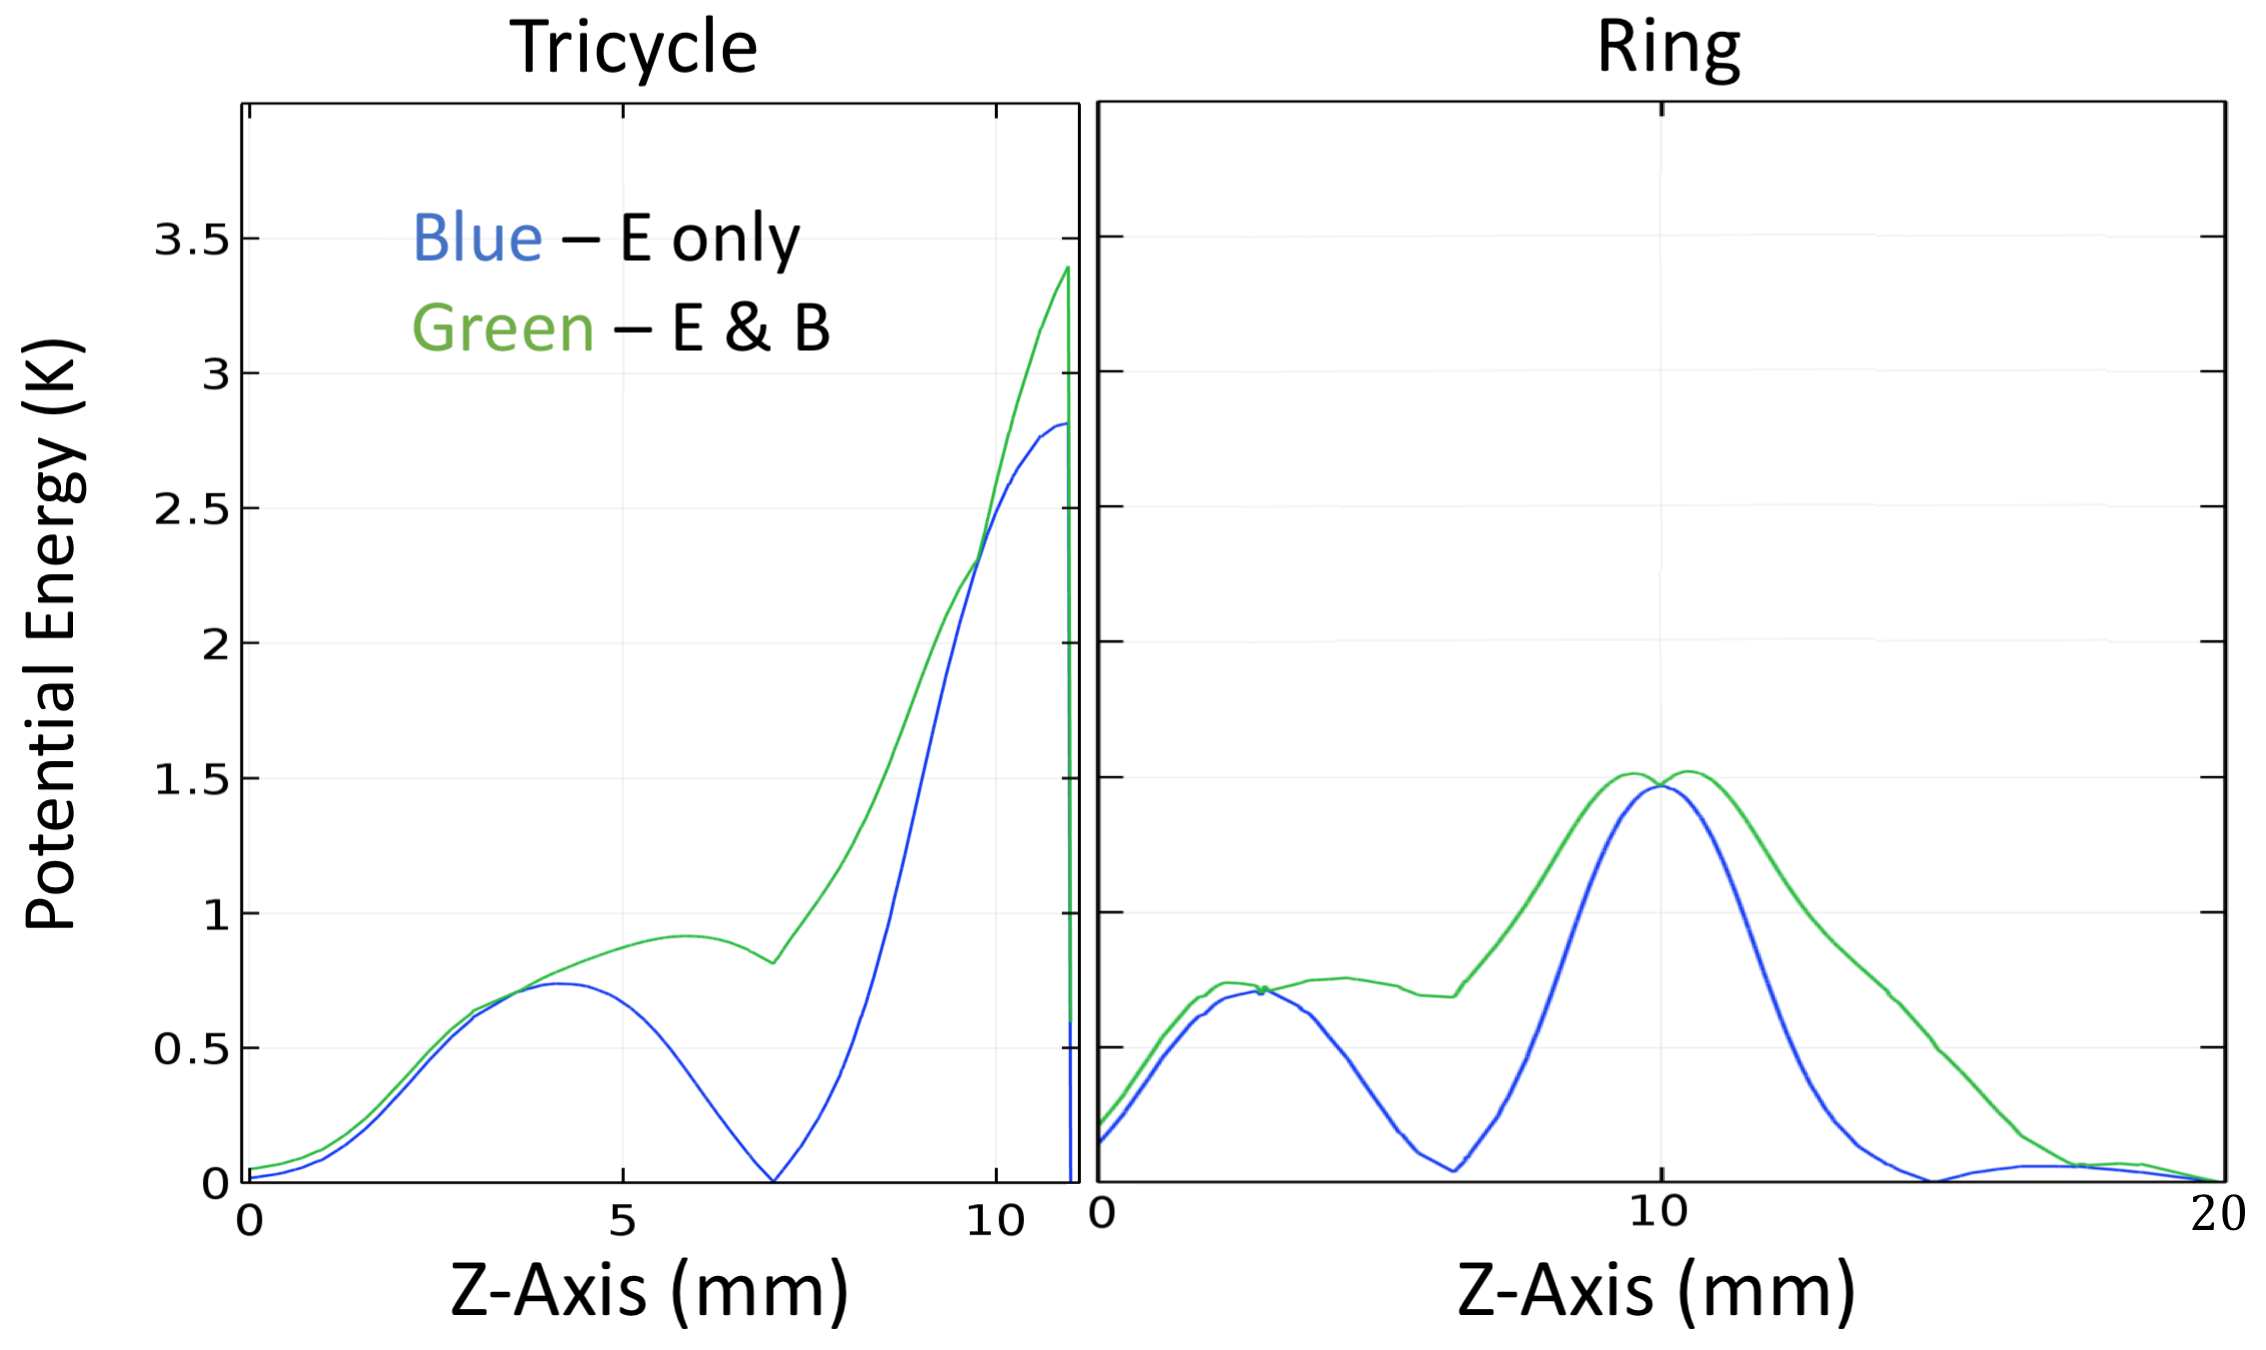
\includegraphics[width=14cm]{LoadingFieldsEB.png}
\caption[On-Axis Loading for Ring and Tricycle]{\label{loadingringtrike}
Potential energy along axis for Ring and Tricycle traps. The trap center is located at $z=10$~mm in both cases. Note the more favorable slope of the loading potential in the vicinity of the trap center for the tricycle trap. Field magnitudes arise from application of $\pm12.5\text{ kV}$ for the Ring trap and also for the Tricycle. In practice almost half this voltage was applied on the Tricycle for optimal operation, perhaps due to arcing effects or nonadiabatic transitions during loading discussed below in Sec.~\ref{loadingtransitions}.
}
\end{figure}

In practice, Fig.~\ref{loadingringtrike} shows what we are able to obtain for loading fields comparing the Ring and Tricycle traps.
Note the role of the magnetic field, which is non-negligible.
The tricycle trap comes much closer to the harmonic ideal discussed above.
For the ring trap, the extra effect of the magnetic field actually depresses the potential energy at the trap center below a wider plateau, making it formally impossible to bring the synchronous molecule to rest at the trap center.
In practice, the experimentally determined ideal application time of loading fields likely corresponds to the synchronous molecule being brought close to rest but out in front of the trap center.
This unideal situation should result in a higher loaded temperature in the ring trap compared with the tricycle trap, $87$~mK compared with $61$~mK in simulation.
In practice however, the measured spectra of molecules in the Ring trap fits better to a thermal distribution and to a lower temperature compared with the tricycle trap, see Fig.~\ref{RingTriSpectrum.png}.
Before discussing this further, we first revisit the process of spectroscopy in these traps.

% SUBSECTION MICROWAVE SPECTROSCOPY
\subsection{Microwave Spectroscopy}

A critical tool for understanding the behavior of populations in our magnetic traps is microwave spectroscopy performed on the parity changing transition between $|f, \frac{3}{2}\rangle$ and $|e, \frac{3}{2}\rangle$ states.
This transition is ideal for spectroscopy, because it has a very small but nonetheless nonzero differential Zeeman shift of $26.6$~MHz/T, which allows molecules to be resolved according to their magnetic field, while also allowing the entire trap to be surveyed over a very narrow bandwidth of microwave frequencies.
The narrowness of the band is crucial for avoiding the complexities associated with the delivery of microwaves to the trapping region.
If it were necessary to instead use microwaves to transfer molecules directly from a trapped to an untrapped state by flipping their magnetic quantum number, $|f, \frac{3}{2}\rangle$ to $|f, -\frac{3}{2}\rangle$, scanning the trap would require scanning the applied microwave frequency between $1.7$ and $16$~GHz.
While this is no problem for the microwave synthesizer itself, obtaining a suitably level passband in the components responsible for delivering the microwaves to the molecules would be unfeasible.
In particular, the microwaves are delivered to the trap using a bias tee setup, nicely described in~\citep[Fig.~5]{stuhl2012uwave}, and the transfer function through the isolation capacitors is particularly troublesome, see Fig.~\ref{broadercoupling.png}.
In contrast, with the entire population sitting below $0.5$~T, only $13$~MHz needs to be scanned out of $1.7$~GHz, and no significant attenuation variation is expected or measured.

\figdave{broadercoupling.png}{Microwave Coupling through Bias Tee}{Microwave transfer function from vacuum feedthrough to magnet surfaces. Large variations are observed across the GHz scale required for performing spectroscopy along $m$-changing transitions, but not on the MHz scale required for $|f, \frac{3}{2}\rangle$ to $|e, \frac{3}{2}\rangle$ spectroscopy.}{10cm}

In addition to the use of microwaves to transfer population, the spectroscopy relies on a few further steps.
First, molecules in the $|e, \frac{3}{2}\rangle$ state remain trapped, and must be removed.
This is done by first applying a bias electric field to allow molecules to escape via avoided crossings, as discussed in Chapter~\ref{chapter:Background}.
In~\cite{stuhl2012uwave}, it was nicely demonstrated that this is effective for removing molecules in the $|e\rangle$ state.
Second, the process is repeated many times, with varying wait times so as to avoid any pathological resonance between the application of microwaves and the oscillation of molecules in the trap, which could result in certain privileged classes of molecule orbits always avoiding the microwaves.
Third, comparison is made between the total laser induced fluorescence with and without the application of the spectroscopic sequence.
When this is done, spectra such as shown in Fig.~\ref{RingTriSpectra.png} are obtained.

\figdave{RingTriSpectrum.png}{Spectra in Ring and Tricycle Trap}{Spectra in the Ring and Tricycle traps after loading with no evaporation. The former was published in \citep[Fig.~3a]{stuhl2012evap}, the latter was collected on Feb.~24, 2014.}{\linewidth}

% SUBSECTION LIMITATIONS TO SPECTROSCOPY
\subsection{Limitations to Spectroscopy}

Inherent in the spectroscopic procedure just described are several key assumptions, which vary in their validity and deserve some further discussion.

\subsubsection{Spatial Sensitivity Variations}

The influence on microwave frequency dependent intensity has already been claimed negligible, but microwave intensity at any given frequency varies significantly across the cloud.
This goes against the rule of thumb that electromagnetic intensity shouldn't vary significantly on lengthscales below a wavelength, $18$~cm in this case.
This is because the microwaves are in the near field regime with respect to the conductors that form the trapping potential.
The microwave fields may to a good approximation be taken to be dominantly electric and equal to the DC electric field distribution generated during loading but with magnitude oscillating at the microwave frequency.
This means that their intensity should vary as shown in Fig.~\ref{NearFieldUWave.png}ab.
In particular, the microwave intensity falls off quickly as molecules approach the openings of the magnets of the Ring trap.
Furthermore, the efficiency of microwave transfer also features a polarization dependence.
Since the $|f,\frac{3}{2}\rangle$ to $|e,\frac{3}{2}\rangle$ transition has $\Delta m=0$, there is a dependence of the Rabi frequency describing the intensity of the microwave drive on the cosine of the angle $\theta$ between the electric and magnetic fields, see panel~(c) of Fig.~\ref{NearFieldUWave.png}.
This ends up favoring molecules on the axis of the trap.

\figdave{NearFieldUWave.png}{Near Field Microwave Intensity in Ring and Tricycle Trap}{The near field intensity close to the (a) Tricycle trap and (b) Ring trap. Colors and contours are relative to the magnitude of the microwave drive, but may be thought of as ranging from $0$ to $100\%$ as color ranges from black to red to yellow to white, with contours at $5\%$ intervals. Colors are comparable between the two traps, assuming the same microwave intensity on the surface of the conductors. These are also the DC field distributions for loading the traps, in which case color ranges from $0$ to $200$~kV/cm with contours every $10$~kV/cm and $25$~kV applied across the magnet surfaces. Rings are $3$~mm apart for the Ring trap and in the Tricycle trap magnets are $2$~mm apart. (c) The angle between electric and magnetic fields is shown, from red, $0$, to blue, $\pi/2$ radians. Magnetic field contours every $500$~G are superposed.}{\linewidth}

In mid 2013, an effort was made to perform spectroscopy along the $|f, \frac{3}{2}\rangle$ to $|e, \frac{1}{2}\rangle$ transition, with the goal of addressing the issue that $|e,\frac{3}{2}\rangle$-state molecules with total energies below the lowest crossing of the $|e,\frac{3}{2}\rangle$ and $|f,\frac{-3}{2}\rangle$ states at $410$~G are unable to find their way out of the trap, see Fig.~\ref{sigmaspec.png}.
The results were quite different from those performed along the $|f, \frac{3}{2}\rangle$ to $|e, \frac{3}{2}\rangle$ transition, perhaps due to polarization differences since this transition would feature dependence on $sin(\theta)$, but more likely reflective of the microwave coupling bandwidth issues discussed above.

\figdave{sigmaspec.png}{Spectroscopy from $|f, \frac{3}{2}\rangle$ to $|e, \frac{1}{2}\rangle$}{Depletion spectroscopy performed by microwave transfer from the $|f, \frac{3}{2}\rangle$ to $|e, \frac{1}{2}\rangle$ state. The dip between $800-1000$~G is likely an artifact of coupling efficiency challenges.}{10cm}

A final point is the spatial dependence of the fluorescence collection system. 

% SUBSECTION LOADED SPECTRA
\subsection{Loaded Spectra}

The obtained spectra in the two traps are compared in Fig.~\ref{RingTriSpectrum.png}.
Several important features are worth discussing here.
First of all, the Ring trap fits nicely to a Maxwell-Boltzmann distribution, which in a linear trapping geometry should scale with magnetic field in the following way:
\begin{equation}
\label{spectralform}
p(B)\propto B^2e^{\mu_B B/kT}.
\end{equation}
The exponential term gives the expected Boltzmann suppression factor as a function of increasing potential energy, while the $B^2$ term is proportional to the volume degeneracy factor.
In other words, the volume corresponding to a magnetic field $B$ within $dB$ is an ellipsoidal shell in the linear trap, whose surface area grows proportionally to $B^2$ since the trap is linear.
Of course there is also the microwave polarization factor to keep in mind, but close to the center of the quadrupole trap, the volume degeneracy factor weighted by polarization selectivity should still grow as $B^2$ and be representative of the population distribution.
Further away from the center however this is a different story.
Molecules might be exploring the region between the central and toroidal traps, but this region is opaque due to polarization.
In the region that is not opaque, close to the axis, there is also a significant change in field gradient that occurs between $1-2$~kG. Above $2$~kG, contour lines are much more closely spaced than below $1$~kG, so that in principle the volume degeneracy factor should be different for the two regions.
One corollary is that a true Maxwell-Boltzmann distribution in this trap ought to feature reduced population in the region above $2$~kG relative to what one would get by fitting the functional form in Eq.~\ref{spectralform}.

In the tricycle trap, the fit is more dubious. 
Points clearly fall below the fit at high magnetic fields, and also seem to lie below at the lowest fields as well.
On the other hand, given that the tricycle trap opens to the environment above $3$~kG, it may be that falling below the Maxwell-Boltzmann fit line is the more natural thing to occur in this situation.
Unlike in the Ring trap where there is no sign of the expected volume enhancement factor that would correspond to plateaus at $1100$~G, the Tricycle trap spectrum shows more agreement as far as its expected deviations from the pure thermal spectrum are concerned.

Regardless of the fitting of distributions, one thing is certain when comparing the Ring and Tricycle traps.
In the latter, many more molecules are confined in a smaller volume.
The Tricycle trap improves upon the Ring by a factor of two in gradient, and both show the majority of their trapped populations lying below $2$~kG, indicating that for the same total population, the spatial density is eightfold enhanced in the Tricycle trap.
As far as actual total numbers are concerned, they are remarkably similar between the two traps, with both featuring similar collection solid angles and similar final numbers of photons detected.

\subsection{}


\section{Spin-Flips During Loading}
\label{loadingtransitions}

\section{Pin Trap}

\section{Other traps in the field}

\section{Spin-flip Losses, Dipolar Enhancements thereof}

\section{Dynamical Phenomenon}

\section{Next Generation Traps}



\bibliographystyle{unsrtDR}	% or "siam", or "alpha", etc.
\bibliography{allrefs}		% Bib database in "allrefs.bib"
\end{document}




